\documentclass[oneside,english,final]{amsbook}
% File soley meant for shared latex macros and imports.
\makeatletter
\DeclareRobustCommand*\cal{\@fontswitch\relax\mathcal}
\usepackage{expl3}
\usepackage{cancel}
\usepackage{fancyvrb}
\usepackage[final]{listings}
\usepackage{multicol}
\usepackage{color}
\usepackage{xcolor}

% following were used in other papers of mine, leaving commented out in
% case I wind up needing one or two of these.
%\usepackage{pdfcolmk}
%\usepackage{supertabular}
%\usepackage{symbolindex}
%\usepackage{amstext}
%\usepackage{amssymb}
%\usepackage{mathtools}
%\usepackage{mathstyle}
%\usepackage{breqn}
%\usepackage{amsmath}
%\usepackage{isomath}
%\usepackage{outline}

\usepackage{xparse}
% Exacting typesetting for SI units.
\usepackage{sistyle}
\usepackage{ifthen}
\usepackage{polynomial}
\usepackage{theoremref}
\usepackage{todonotes}
\usepackage{fancyhdr}
\pagestyle{fancy}
\usepackage[active]{srcltx}
\usepackage{babel}
\usepackage{fixltx2e}
\usepackage{enumitem}
\usepackage{amsthm}
\usepackage{wasysym}
\usepackage[all]{xy}
\PassOptionsToPackage{normalem}{ulem}
\usepackage{ulem}
\usepackage{empheq}
\usepackage{xfrac}
\usepackage{bytefield}
\usepackage{cite}
\usepackage{fixme}


\usepackage{marginnote}

\usepackage{polynom}
\usepackage{exscale}
\usepackage{url}
\usepackage{tikz}

% Import in the whole kitchen sink for TiKz
\usetikzlibrary{arrows,backgrounds,matrix,
  plothandlers,plotmarks,shadings,shadows,
  svg.path,topaths,through,trees,fit,fadings,
  er,circuits,calc,automata,intersections, patterns,positioning,
  decorations.pathmorphing, decorations.pathreplacing,
  decorations.markings, decorations.footprints, decorations.shapes,
  decorations.text, decorations.fractals, chains}

\usepackage[unicode=true,
            bookmarks=true,bookmarksnumbered=false,
            bookmarksopen=true,bookmarksopenlevel=6,
            breaklinks=false,pdfborder={0 0 1},
            backref=page,colorlinks=true] {hyperref}

\usepackage{glossaries}

\setcounter{errorcontextlines}{10}
%\DeclareMathOperator{\rank}{rank}

\newenvironment{sqcases}{%
  \matrix@check\sqcases\env@sqcases
}{%
  \endarray\right.%
}
\def\env@sqcases{%
  \let\@ifnextchar\new@ifnextchar
  \left\lbrack
  \def\arraystretch{1.2}%
  \array{@{}l@{\quad}l@{}}%
}


\providecolor{nix_color_TODO}{rgb}{0.75,0,0}
\providecolor{nix_color_thought}{rgb}{0,0,0.5}
\newcommand{\thought}[1]{{\texorpdfstring{\color{nix_color_thought}{#1}}{}}}

%% Until I find the official one, this denotes LaTeX3.
\newcommand\LaTeXThree{$\LaTeX{}_3$}

\newcommand\keyword[1]{\emph{#1}}
\newcommand{\ba}{\begin{array}}
\newcommand{\ea}{\end{array}}
\newcommand{\bq}{\begin{quote}}
\newcommand{\eq}{\end{quote}}
\newcommand{\bt}{\begin{tabular}}
\newcommand{\et}{\end{tabular}}
\newcommand{\bi}{\begin{itemize}}
\newcommand{\ei}{\end{itemize}}
\newcommand{\be}{\begin{enumerate}}
\newcommand{\ee}{\end{enumerate}}



% For HTML anchors I believe.
\newcommand{\anchor}[2]{#2}
\newcommand{\lb}{[\![}
\newcommand{\rb}{]\!]}
\newcommand{\db}[1]{\lb#1\rb}


\newcommand\TODO[1]{{({\bf $\spadesuit$~TODO:} \texorpdfstring{\color{nix_color_TODO}{\em #1}}{}})}

\newcommand{\indextt}[1]{\index{#1@@{\tt #1}}}
\newcommand{\indexsyn}[1]{\index{#1@@{\it #1}}}
\newcommand{\indexmodule}[1]{\index{#1@@{\tt #1} (module)}}
\newcommand{\indextycon}[1]{\index{#1@@{\tt #1} (datatype)}}
\newcommand{\indexsynonym}[1]{\index{#1@@{\tt #1} (type synonym)}}
\newcommand{\indexclass}[1]{\index{#1@@{\tt #1} (class)}}
\newcommand{\indexdi}[1]{\index{#1@@{\tt #1} (class)!derived instance}}
\newcommand{\indexnote}[1]{#1n}
\newcommand{\emptystr}{[\,]}
\newcommand{\ignorehtml}[1]{#1}
\def\skipline{\vskip 1em}
\newsavebox{\fmbox}


\newcommand{\bkq}{\mbox{\tt \char'022}} % (syntax) backquote char
\newcommand{\bkqB}{\bkq\hspace{-.2em}} % (syntax) backquote char (Before)
\newcommand{\bkqA}{\hspace{-.2em}\bkq}% (syntax) backquote char (After)

\newcommand\sq[1]{[\,#1\,]}

% denotional semantics
\newcommand{\den}[2]{{\cal #1}\db{#2}\,}
\newcommand{\denote}[3]{\[\ba{c} {\cal #1} : #2 \\[1 ex] #3 \ea\]}


% mathy things
\newcommand{\x}{\times}













%%%%%%%%%%%%%%%%%%%%%%%%%%%%%% Textclass specific LaTeX commands.
\numberwithin{section}{chapter}
\numberwithin{equation}{section}
\numberwithin{figure}{section}
\newlength{\lyxlabelwidth}      % auxiliary length 
\numberwithin{table}{section}
\theoremstyle{plain}
\newtheorem{thm}{\protect\theoremname}
  \theoremstyle{definition}
  \newtheorem{example}[thm]{\protect\examplename}
  \theoremstyle{remark}
  \newtheorem{rem}[thm]{\protect\remarkname}
  \theoremstyle{remark}
  \newtheorem{note}[thm]{\protect\notename}
  \theoremstyle{plain}
  \newtheorem{question}[thm]{\protect\questionname}
  \theoremstyle{remark}
  \newtheorem{claim}[thm]{\protect\claimname}
  \theoremstyle{definition}
  \newtheorem*{example*}{\protect\examplename}
  \theoremstyle{remark}
  \newtheorem{notation}[thm]{\protect\notationname}
  \theoremstyle{remark}
  \newtheorem*{note*}{\protect\notename}
  \theoremstyle{definition}
  \newtheorem{defn}[thm]{\protect\definitionname}
  \theoremstyle{plain}
  \newtheorem{fact}[thm]{\protect\factname}
\newcommand{\strong}[1]{\textbf{#1}}
\usepackage{xunicode}
  \providecommand{\claimname}{Claim}
  \providecommand{\definitionname}{Definition}
  \providecommand{\examplename}{Example}
  \providecommand{\notationname}{Notation}
  \providecommand{\notename}{Note}
  \providecommand{\questionname}{Question}
  \providecommand{\remarkname}{Remark}
  \providecommand{\factname}{Fact}
\providecommand{\theoremname}{Theorem}





%\newcommand\Acronym[2]{#2 (#1)}


\ExplSyntaxOn


\DeclareDocumentCommand \Acronym { l m } {
  #2~(#1)
%  \def\NoDocumentation{}
%  \IfNoValueTF {#1} { % Default case, docs at #2.pdf
%    \@pkg{#2}~\pkgdocs{#2}{#2}
%  }{
%    \if_meaning:w #1 \NoDocumentation
%    \@pkg{#2}        % Package has no known documentation.
%    \else:
%    \@pkg{#2}~\pkgdocs{#2}{#1} % Documentation at some other filename.
%    \fi:
%  }
}
\ExplSyntaxOff

\DeclareMathAccent{\ring}{\mathalpha}{operators}{"17}
\providecommand*{\angs}{%
  \ensuremath{\smash{\mathrm{\ring A}}}}

\providecommand*{\ohm}{%
  \ensuremath{\mathrm{\Omega}}}

\providecommand*{\degree}{%
  \ensuremath{^\circ}}

\providecommand*{\celsius}{%
  \ensuremath{\mathrm{^\circ C}}}

\providecommand*{\micro}{%
  \ensuremath{\mu}}

\providecommand*{\unit}[1]{%
  \ensuremath{\mathrm{\,#1}}}

\providecommand*{\ped}[1]{%
  \ensuremath{_\mathrm{#1}}}
\providecommand*{\ap}[1]{%
  \ensuremath{^\mathrm{#1}}}



\makeatother
%%% Local Variables: 
%%% mode: latex
%%% TeX-master: osdev
%%% End: 
\glsSetCompositor{-}
\newcommand\register[1]{\texttt{#1}}
\def\acronymtype{acronym}
\newglossary[alg]{acronym}{acr}{acn}{\acronymname}
\makeglossaries
\glsenablehyper
\newcommand\cn{{\small{\ap{\textbf{[\textit{citation-needed}]}}}}}
\newcommand\newmnemonic[2]{}
\glsaddall[types={main,\acronymtype}]
\newmnemonic{ADD}{addition}
\newmnemonic{SUB}{subtract}
\newmnemonic{DIV}{division}
\newmnemonic{MUL}{multiplication}
\newmnemonic{MOV}{move}
\newmnemonic{NOP}{no operation}

\newmnemonic{RETF}{far return}
\newmnemonic{RET}{near return}%or just Return...

\newmnemonic{LGDT}{load global descriptor table}
\newmnemonic{SGDT}{store global descriptor table}

\newmnemonic{SFENCE}{store fence}

\newacronym{acpi}{ACPI}{Advanced Control~and~Power Interface}
\newacronym{rsdt}{RSDT}{What is it?}
\newacronym{xsdt}{XSDT}{What is it?}
\newacronym{cpu}{CPU}{Central Processing Unit}
\newacronym{usb}{USB}{Universal Serial Bus}
%Also could be "personal computer", but we will need to talk about
%the program counter much more then the simplified term 'personal computer'.
\newacronym{pc}{PC}{Program Counter}
\newacronym{gdtr}{\register{GDTR}}{Global Descriptor Table Register}
\newacronym{gdt}{GDT}{Global Descriptor Table}
\newacronym{bios}{BIOS}{Basic~Input/Output~System}

%%% Local Variables: 
%%% mode: latex
%%% TeX-master: "osdev"
%%% End: 

\newglossaryentry{bit}{name=bit, description={Binary toggle, there are 8
    bits to a byte}}  

\newglossaryentry{nibble}{name=nibble,
  description={Half of a byte, four bits}}

\newglossaryentry{byte}{name=byte,description={A grouping of 8 bits on all
    modern architectures. Some unusual architectures such as MIX assign
    different numbers of bits to a byte.\cn}}

\newglossaryentry{word}{name=word,
  description={Equivalent of two bytes}}

\newglossaryentry{double word}{name=double~word,
  description={Equivalent of four bytes}}

\newglossaryentry{quad word}{name=quad~word,
  description={Equivalent of eight bytes}}

\newglossaryentry{x86}{name=x86, description={assembler thing}}

\newglossaryentry{x86-64}{name=x86-64,description={Extension of the x86 CPU
    architecture to 64 bits}}

\newglossaryentry{page fault}{name=page~fault,description={Occurs when
    interrupt~14 fires}}

\newglossaryentry{little endian}{%
  name=little~endian, description={Opposite of big endian\todo{summarize
      this... how!}}}
%%% Local Variables: 
%%% mode: latex
%%% TeX-master: "osdev"
%%% End: 


\glsaddall

\newenvironment{technote}{%
    \skipline\par
    \begin{tikzpicture}
    \node[rectangle,minimum width=0.9\textwidth] (m)
    \bgroup\begin{minipage}{0.85\textwidth}$\!\!\!$\textbf{TechNote:} \ignorespaces%
}{%
    \end{minipage}\egroup;
    \draw[dashed] (m.south west) rectangle (m.north east);
    \end{tikzpicture}
    \skipline
}

\newenvironment{testidea}{%
    \skipline\par
    \begin{tikzpicture}
    \node[rectangle,minimum width=0.9\textwidth] (m)
    \bgroup\begin{minipage}{0.85\textwidth}$\!\!\!$\textbf{TestIdea:} \ignorespaces%
}{%
    \end{minipage}\egroup;
    \draw (m.south west) rectangle (m.north east);
    \end{tikzpicture}
    \skipline
}

%\newcommand\technote[1]{\emph{\tiny{Technical~note: #1}}}

\title{Art of Operating System Development}
%\address{i@nixeagle.org}

\begin{document}
\maketitle
\frontmatter
\tableofcontents
\mainmatter

\part{First things}
{\small\textit{Note that this book will be seperated into multiple parts. The
  first few chapters will cover a general overview of the subject and
  various aspects of the boot sequence.}}
\chapter{Foreword/Introduction}
We intend to explain how to develop an operating system on the \gls{x86}
{architecture}\footnote{This includes the \gls{x86-64} variants. Later in
  the far far future discussion on other machine types may be included.}.
\section{Data sizes}
Explain \gls{bit}, \gls{nibble}, \gls{byte}, \gls{word}, 
\gls{double word}, and \gls{quad word}.

\begin{figure}[h]%
  \caption{\protect\Gls{byte}}
  \label{fig:byte}
  \skipline
  \begin{bytefield}{8}
    \bitheader[b]{0-7} \\
    \wordbox{1}{Byte}
  \end{bytefield}
\end{figure}

A machine \gls{double word} is 32 bits.\cn So we are clear, that is 4
bytes.

\begin{figure}[h]%
  \caption{\protect\Gls{double word}\relax}
  \label{fig:double-word}
  \skipline
  \begin{bytefield}{32}
    \bitheader[b]{0,7,8,15,16,23,24,31} \\
    \bitbox{8}{} \bitbox{8}{} \bitbox{8}{} \bitbox{8}{}
  \end{bytefield}
\end{figure}

There are various other terms including \gls{nibble}, \gls{word} and \gls{quad word}. We
will discuss these when they come up. \todo{where?}

\section{Which Endian?}
% further explain what endian is and how we will handle data sizes
As the \gls{x86} architecture is \gls{little endian}, all of our figures
and notation will also be little~endian. So when talking about where
a~\gls{bit} is~in a~\gls{byte} we will start counting from the~right
to~left.\cite{wikipedia_endianness_2011,cohen_holy_war_1980} Looking at
figure \ref{fig:byte}, we notice that the 0\ap{th} bit is located to the far right
and the 7\ap{th} bit is located to the far left.

The attentive reader should note that we have started counting at
\emph{zero} instead of \emph{one}. This is the traditional way for computer
scientists to count.\cn\todo{I'd really like to rewrite this with a better
  word flow\ldots.}


\chapter{Boot Loader}
On x86 systems the \gls*{bios} starts execution at physical address
\verb|0x7c00|. The \gls*{cpu} will get control operating in \gls{real
  mode}. Real mode is~very limited, only~1MB of~memory may be
accessed.\cn\todo{Check that real mode memory limits are correct}

\begin{technote}%
  The contents of the \register{DL}~register indicate which drive contains
  the~loaded boot-sector. Store this number for~later reference if
  the~kernel is~to~handle being booted from a~machine with more than
  one~drive.
\end{technote}

Either the \gls{boot loader} or the \keyword{kernel} has to~bring
the~CPU into protected mode.

\Gls{byte addressing} means memory access is~accessed as~a~sequence
of~bytes.\cite{intel-v3A}

An \gls{address space} is the set of addressable bytes that can be
selected at a given time.\cite{intel-v3A}

Since the~whole memory space cannot be~accessed at~one~time on a~32bit
system the concept of~\keyword{segments} was invented. A~segment is~just
a~named address-space. There are six segment registers on a 32bit
system.\cite[3-4]{intel-v1}\todo{Write something about how many of these
  exist on 64 bit systems.} A dedicated segment can be assigned to the
\keyword{stack} as well as to the currently executing code. \todo{Discuss
  assembly level segment syntax, both intel and gas versions.}



%\cite{intel-x86-vol2A}
\chapter{GDT}
The \gls*{gdtr} is a machine register that serves as a pointer to the linear
address location of the \gls*{gdt}.

Is not considered a segment. Only the LDT and TSS are
segments.\cite[2.1.2]{intel-v3A}

LGDT is the assembly mnemonic for loading a value to the \gls*{gdtr}
register\todo{Expand this explaining how to use the LGDT assembler
  instruction. Might need moved to a later part of this book.}.

\gls*{gdtr} is an oddly shaped machine register that acts as a pointer
containing either 48 bits or 80 bits depending on if a 32 bit mode or 64
bit mode is in use. Figure \ref{fig:GDTR} shows the layout of this machine
register\todo{We have this repeated twice in different ways, see first
  paragraph.}.\cn

There are four system descriptor registers: \register{GDTR},
\register{IDTR}, \register{LDTR}, and
\register{TR}.\cite[2.1.6.1]{intel-v3A}

On segmentation, there is no way to disable segmentation on
32~bit\cite[3.2.4]{intel-v3A} x86~processors.\cite[3.1]{intel-v3A} For
the 64bit architectures segmentation is largely unused. Intel specification
states that a processor in 64~bit mode will not do runtime segment limit
checks.\cn

Paging is optional.\cn

\begin{testidea}%
  Verify memory size reading is correct.\par
  After GDT is setup, attempt to set the last byte of reachable memory to
  $0xE$ and attempt to read it back.
\end{testidea}
\section{Basic Flat Memory Model}
Simplest way to setup segmentation on x86 architectures. Assumes that the
physical disk is a fixed size regardless of the actual physical
disk\todo{Duck was having a hard time understanding what was meant by
  this, rewrite/improve.}. No general protection faults will be generated.\cn

Two segment descriptors that indicate the whole address space\footnote{On
  32 bit systems this is 4GB.} is usable must be created. The initial state
of the \register{DS}~data segment after initializing this setup will be 0.

\begin{figure}[h]
  \caption{GDTR}
  \label{fig:GDTR}
  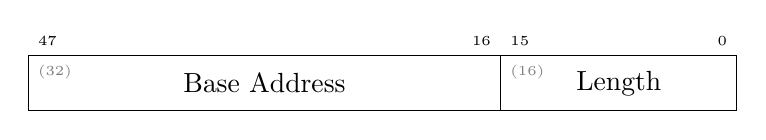
\begin{tikzpicture}%
    \draw (0,0) rectangle 
      node[pos=0.5]{Base Address} (6,2em) rectangle 
      node[pos=0.5]{Length} (9,0);
    \node[above right] at (0,2em) {\tiny{47}};
    \node[above left] at (6,2em) {\tiny{16}};SR  \node[above right] at (6,2em) {\tiny{15}};
    \node[above left] at (9,2em) {\tiny{0}};
    \node [below right,color=gray] at (0,2em) {\tiny{(32)}};
    \node [below right,color=gray] at (6,2em) {\tiny{(16)}};
  \end{tikzpicture}
\end{figure}


%\begin{tikzpicture}%
%  \node [rectangle,draw] {GDTR};
%  \node [above right] at (0,1em) {\tiny{47}};
%\end{tikzpicture}

% Maybe useful... we shall see. #1=lowbit, #2=highbit, #3=width, #4=text.
% if we want to use it, don't forget the greyed out number in the upper
% left corner.
%\def\mythingie#1#2#3#4{%
%  \def\mywidth{#3}
%  \node[rectangle,draw,align=center,minimum height=2em,minimum width=\mywidth] {#4} 
%    node[above left=1em and \mywidth/2-0.5cm]{\tiny{#2}}
%    node[above right=1em and \mywidth/2-0.5cm]{\tiny{#1}}}
%\tikz\mythingie{16}{47}{4cm}{GDT};
%\tikz\mythingie{0}{15}{2cm}{blah};

\chapter{PIT}
\section{CMOS}
\chapter{APIC}
\chapter{ACPI}
A machine independent method of configuring various input and output
devices.\cn Detecting if a computer has \gls*{acpi} support involves
looking in specific memory regions for the string \verb|"RSP PTR "|.\cn
Finding this on a 16 byte boundary marks the start of the RSPT which is
used for finding other ACPI tables.\cn

Checksum fields in all the tables are a single byte that when added to all
the other bytes in the table, the whole table will sum to
0.\cite[Table~6-33]{acpi-spec4a}

\chapter{IRQ}
\chapter{ISR}
\chapter{Keyboard driver}
\section{Interrupt based}
\section{Poll based}

\chapter{Memory Management}
\chapter{Networking}
Want to cover how to write a workable TCP/IP stack.
\chapter{Paging}
\chapter{Context Switching}
\chapter{Userland}
\chapter{multi tasking}
\chapter{Threading}
\chapter{Locking}
\section{Mutex}
\chapter{Linker files}
\chapter{Testing}
\chapter{64 bit x86}
\chapter{Multiboot spec}
\chapter{PCI}
\chapter{USB}
\chapter{CPUID}

\chapter{FAQ} {\small\textit{This chapter will not exist in this form in
    the 1.0 version of this book. The intent here is simply to indicate
    questions that ought to have answers. The porported
    answers to the questions in this chapter should be treated with care
    unless proper citations are given. Again in due time various questions
    and answers will wind up in the book text proper.}}
\section{What is a reliable way to cause a reboot in x86 assembler?}

Just load a 0-sized IDT and interrupt.\footnote{Does not work in virtual
  box and on some hardware.}\cn Also possibly look at
\url{https://github.com/RockerMONO/dux/blob/master/src/metodo/i386/hal/shutdown.c}


\section{How do I cause a triple fault?}

You can't without interrupts setup. \todo{add more!} \marginnote{foobar}[1em]

\section{Why can't I disable interrupts?}

\section{Does anything call sti?}

\section{Is cli run in ring0?}

\section{How much memory can a x86 processor address in real mode?}

\section{Why can't I pop the \register{CS} register?}
Changing running code would be a JMP\ldots so yea I imagine setting the
program counter/whatever segment register you use for code\ldots (I think
cs is mandatory\ldots not sure)\ldots is a simple matter of doing a far
jump.\cn

\section{How do I read from a FAT16 file format?}

\section{Why is a higher half kernel recommended?}
At least recommended by osdev wiki\ldots from what the author understands\ldots.

\section{What is the System V ABI?}

\section{How does canonical naming work?}

\section{What is an ABI for?}

\section{What is Long mode on x86\_64?}

\section{How do I change video modes on x86 hardware?}
Only reasonable way to do this on most hardware is to go through
\emph{vm86} and real mode \emph{VBE interrupts}\cn. 

OTHER

Leave BDA and IVT alone.

Always best to load your kernel at 1MB.


on 32bit x86 machines EAX always contains the return value.

\appendix
\part{Appendix}

\bibliographystyle{plainurl}
\nocite{*}
\bibliography{osdev}

\printglossaries

\listoffigures
\listoftables
\end{document}
%%% Local Variables: 
%%% mode: latex
%%% TeX-master: t
%%% End: 
